\documentclass[a4paper,10pt]{jsarticle}

% レイアウト
\setlength{\textwidth}{\fullwidth}
\setlength{\textheight}{39\baselineskip}
\addtolength{\textheight}{\topskip}
\setlength{\voffset}{-0.5in}
\setlength{\headsep}{0.3in}
\pagestyle{myheadings}

% パッケージ
\usepackage[dvipdfmx]{graphicx}
\usepackage{amsmath,amssymb,epsfig}
\usepackage{bm}
\usepackage{ascmac}
\usepackage{pifont}
\usepackage{multirow}
\usepackage{enumerate}
\usepackage{cases}
\usepackage{type1cm}
\usepackage{cancel}
\usepackage{url}
\usepackage[dvipdfmx]{color}
\usepackage{listings,jlisting}
% 大きな中括弧
\usepackage{cases}

% 定義
\DeclareMathOperator*{\argmin}{arg\,min}
\DeclareMathOperator*{\argmax}{arg\,max}
\def\vec#1{\mbox{\boldmath$#1$}}
\def\R{{\Bbb R}}

% カウンタの設定
\setcounter{section}{0}
\setcounter{subsection}{0}
\setcounter{subsubsection}{0}
\setcounter{equation}{0}

% キャプションの図をFigに変更
\renewcommand{\figurename}{Fig.}
\renewcommand{\tablename}{Tab.}

% 式番号を式(章番号.番号)に
% \makeatletter
% \renewcommand{\theequation}{\arabic{section}.\arabic{equation}}
% \@addtoreset{equation}{section}
% \makeatother

% プログラムに色をつける
\usepackage{color}

\definecolor{codegreen}{rgb}{0,0.6,0}
\definecolor{codegray}{rgb}{0.5,0.5,0.5}
\definecolor{codepurple}{rgb}{0.58,0,0.82}
\definecolor{backcolour}{rgb}{0.95,0.95,0.92}

\lstdefinestyle{mystyle}{
    backgroundcolor=\color{backcolour},
    commentstyle=\color{codegreen},
    keywordstyle=\color{magenta},
    numberstyle=\tiny\color{codegray},
    stringstyle=\color{codepurple},
    basicstyle=\footnotesize,
    breakatwhitespace=false,
    breaklines=true,
    captionpos=b,
    keepspaces=true,
    numbers=left,
    numbersep=5pt,
    showspaces=false,
    showstringspaces=false,
    showtabs=false,
    tabsize=2
}

\lstset{style=mystyle}

% % ドキュメントの開始
\begin{document}

\section{実行方法}
\subsection{動作環境}
LinuxのディストリビューションのひとつであるUbuntuで動作を確認している.
Ubuntuで動作させるための必要なアプリケーションは以下の通りである.

\begin{lstlisting}[basicstyle=\ttfamily\footnotesize, language=Bash, frame=single, firstnumber=1, numbers=left, breaklines=true]
sudo apt-get install build-essential
sudo apt-get install cmake
sudo apt-get install meshlab
\end{lstlisting}

コンパイル時に必要なビルドシステムはbuild-essentialとcmakeが必要であり,生成されたstlのデータ確認のためmeshlabというアプリケーションを用いている.

Visual Studioでのコンパイルも可能であるが,その場合Struct.hの最初の記述を変更する.

\begin{lstlisting}[basicstyle=\ttfamily\footnotesize, language=C, frame=single, firstnumber=4, numbers=left, breaklines=true]
#define _CRT_SECURE_NO_DEPRECATE
#include <stdio.h>
#include <stdlib.h>
#define _USE_MATH_DEFINES
#include <math.h>
\end{lstlisting}

\subsection{ファイル構造}
このzipの中のファイル構造を示す.

\begin{lstlisting}[basicstyle=\ttfamily\footnotesize, language=Bash, frame=single, firstnumber=1, numbers=left, breaklines=true]
.
├── CMakeLists.txt
├── Struct.h
├── document
│  └── document.pdf
├── kadai.h
├── kadai1A.cpp
├── kadai1A.h
├── kadai2A.cpp
├── kadai2A.h
├── main.cpp
└── plot
    ├── Tetra-Triprism.stl
    ├── Tetra01.stl
    ├── Triprism01.stl
    └── tetra_point.dat
\end{lstlisting}
tetra\_point.datが各立体の頂点の初期位置が格納されたデータであり,Tetra01.stlとTriprism01.stlが課題1の結果,Tetra-Triprism.stlが課題2の結果である.

\subsection{コンパイル方法と実行方法}

\begin{lstlisting}[basicstyle=\ttfamily\footnotesize, language=Bash, frame=single, firstnumber=1, numbers=left, breaklines=true]
mkdir build
cd build
cmake ..
make
./実行ファイル名
\end{lstlisting}

\section{実装した関数の説明}
\subsection{課題1}
指定された点から四面体と三角柱を作成するために実装した関数を示す.

\begin{lstlisting}[basicstyle=\ttfamily\footnotesize, language=C, frame=single, numbers=none, breaklines=true]
void InputDatFile(POINT p[], char *fname, double loop);
\end{lstlisting}

\begin{itemize}
 \item 立体用データを外部ファイルから読み込み配列pに格納する.
\end{itemize}

\begin{lstlisting}[basicstyle=\ttfamily\footnotesize, language=C, frame=single, numbers=none, breaklines=true]
void set_tetra(double vs[][VEC_SIZE]);
\end{lstlisting}

\begin{itemize}
 \item データから立体を表す座標を2次元配列に格納(四面体用)
\end{itemize}

\begin{lstlisting}[basicstyle=\ttfamily\footnotesize, language=C, frame=single, numbers=none, breaklines=true]
void set_triprism(double vs[][VEC_SIZE], double h);
\end{lstlisting}

\begin{itemize}
 \item データから立体を表す座標を2次元配列に格納(三角柱用)
\end{itemize}

\begin{lstlisting}[basicstyle=\ttfamily\footnotesize, language=C, frame=single, numbers=none, breaklines=true]
void norm_triangle(double n[VEC_SIZE], double v0[VEC_SIZE], double v1[VEC_SIZE], double v2[VEC_SIZE]);
\end{lstlisting}

\begin{itemize}
 \item 外向き法線ベクトル作成する
 \item 法線ベクトルを求めた結果は配列nに格納される
\end{itemize}

\begin{lstlisting}[basicstyle=\ttfamily\footnotesize, language=C, frame=single, numbers=none, breaklines=true]
void prStlProlog(char *label, FILE *fp);
\end{lstlisting}

\begin{itemize}
 \item STL形式の開始行を作成
\end{itemize}

\begin{lstlisting}[basicstyle=\ttfamily\footnotesize, language=C, frame=single, numbers=none, breaklines=true]
void prStlEpilog(char *label, FILE *fp);
\end{lstlisting}

\begin{itemize}
 \item STL形式の終了行を作成
\end{itemize}

\begin{lstlisting}[basicstyle=\ttfamily\footnotesize, language=C, frame=single, numbers=none, breaklines=true]
void prStlFacet(double n[VEC_SIZE], double v0[VEC_SIZE], double v1[VEC_SIZE], double v2[VEC_SIZE], FILE *fp);
\end{lstlisting}

\begin{itemize}
 \item STL形式の三角形パッチを作成
 \item 頂点と外向き法線ベクトルを引数に
\end{itemize}

\begin{lstlisting}[basicstyle=\ttfamily\footnotesize, language=C, frame=single, numbers=none, breaklines=true]
void CombinationTetra(double vs[][VEC_SIZE], FILE *fp);
\end{lstlisting}

\begin{itemize}
 \item 外向き法線方向に右ねじが進む方向の点の組み合わせ作成(四面体用)
\end{itemize}

\begin{lstlisting}[basicstyle=\ttfamily\footnotesize, language=C, frame=single, numbers=none, breaklines=true]
void prStlTetra(double vs[][VEC_SIZE], char *label);
\end{lstlisting}

\begin{itemize}
 \item STL形式の四面体作成
\end{itemize}

\begin{lstlisting}[basicstyle=\ttfamily\footnotesize, language=C, frame=single, numbers=none, breaklines=true]
void CombinationTriprism(double vs[][VEC_SIZE], FILE *fp);
\end{lstlisting}

\begin{itemize}
 \item 外向き法線方向に右ねじが進む方向の点の組み合わせ作成(三角柱用)
 \item 外向き法線方向に右ねじが進む順番になるようすべて列挙している
\end{itemize}

\begin{lstlisting}[basicstyle=\ttfamily\footnotesize, language=C, frame=single, numbers=none, breaklines=true]
void prStlTriprism(double vs[][VEC_SIZE], char *label);
\end{lstlisting}

\begin{itemize}
 \item STL形式の三角柱作成
\end{itemize}

\begin{lstlisting}[basicstyle=\ttfamily\footnotesize, language=C, frame=single, numbers=none, breaklines=true]
void stlb_k01(double tt[TETRA_V_NUM][VEC_SIZE], double tp[TRIPRISM_V_NUM][VEC_SIZE]);
\end{lstlisting}

\begin{itemize}
 \item 四面体と三角柱をSTL形式でそれぞれ作成 (課題2Aの1)
\end{itemize}

\subsection{課題2}

\begin{lstlisting}[basicstyle=\ttfamily\footnotesize, language=C, frame=single, numbers=none, breaklines=true]
double GetRandom(double min,double max, int digit);
\end{lstlisting}

\begin{itemize}
 \item 範囲と所望の小数点以下の桁数を指定して乱数を得る
\end{itemize}

\begin{lstlisting}[basicstyle=\ttfamily\footnotesize, language=C, frame=single, numbers=none, breaklines=true]
AXIS randCoordinateAxis();
\end{lstlisting}

\begin{itemize}
 \item 任意の原点位置と任意の軸方向を持つ新たな座標系をランダムに作成
 \item 課題1Bで作成したものと同じ原理で結果を得ている
\end{itemize}

\begin{lstlisting}[basicstyle=\ttfamily\footnotesize, language=C, frame=single, numbers=none, breaklines=true]
void CalcRotationMat(POINT input[], POINT output[], double rotation_mat[][VEC_SIZE], int loop);
\end{lstlisting}

\begin{itemize}
 \item 引数にとった変換行列を立体を表現している座標群に施す
\end{itemize}

\begin{lstlisting}[basicstyle=\ttfamily\footnotesize, language=C, frame=single, numbers=none, breaklines=true]
void TransformPosition(char *label, FILE *fp);
\end{lstlisting}

\begin{itemize}
 \item 取る引数(label)によって欲しい立体(四面体か三角柱用)をランダムな座標系で作成
\end{itemize}

\begin{lstlisting}[basicstyle=\ttfamily\footnotesize, language=C, frame=single, numbers=none, breaklines=true]
void TransformPositionAll(char *label);
\end{lstlisting}

\begin{itemize}
 \item 課題2Aの2を実行する
\end{itemize}

\section{結果}
それぞれの課題で結果を示す.
\subsection{課題1}
四面体を出力した結果をFig.~\ref{fig:四面体を作成した結果},三角柱を出力した結果をFig.~\ref{fig:三角柱を作成した結果}に示す.
\begin{figure}[b]
  \centering
  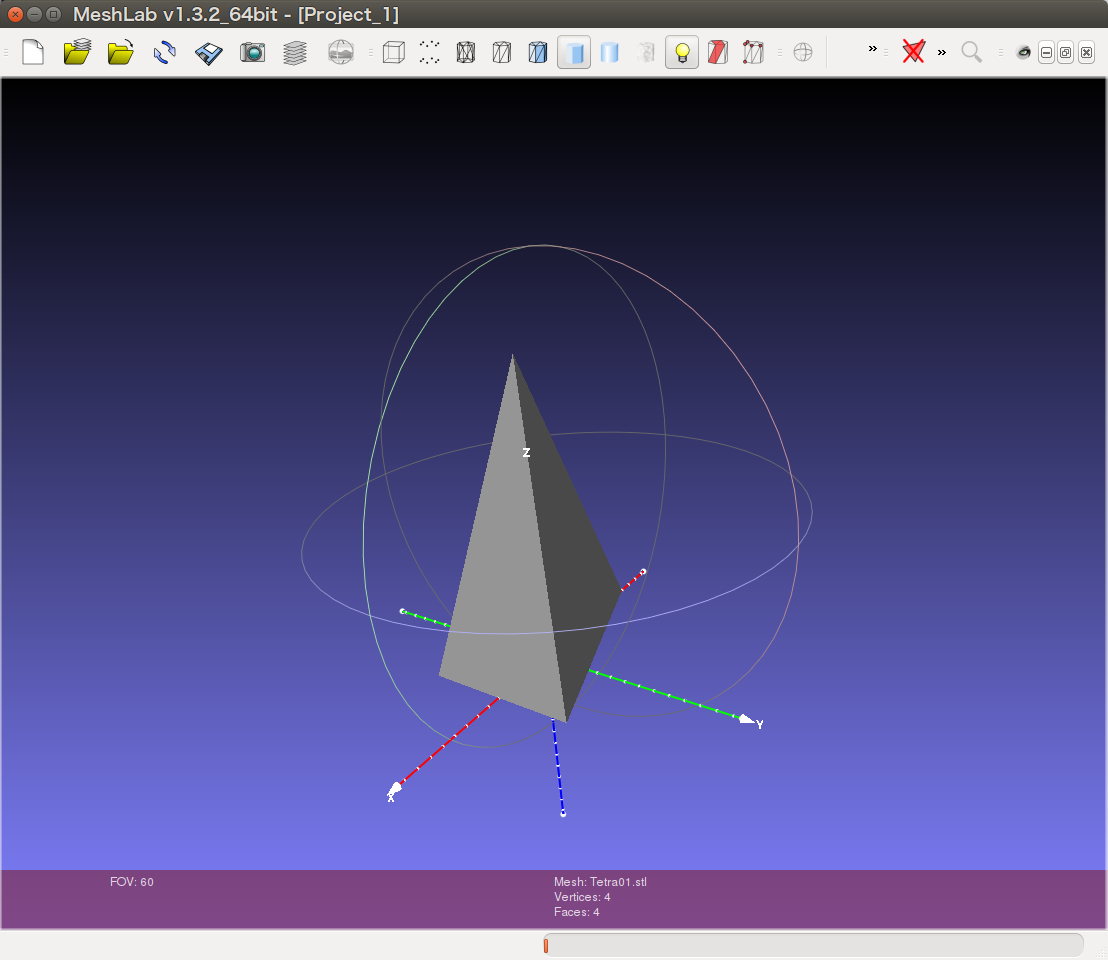
\includegraphics[width=100mm, bb = 0 0 1108 960]{fig/png/Tetra01.png}
  \caption{四面体を作成した結果}
  \label{fig:四面体を作成した結果}
\end{figure}

\begin{figure}[t]
  \centering
  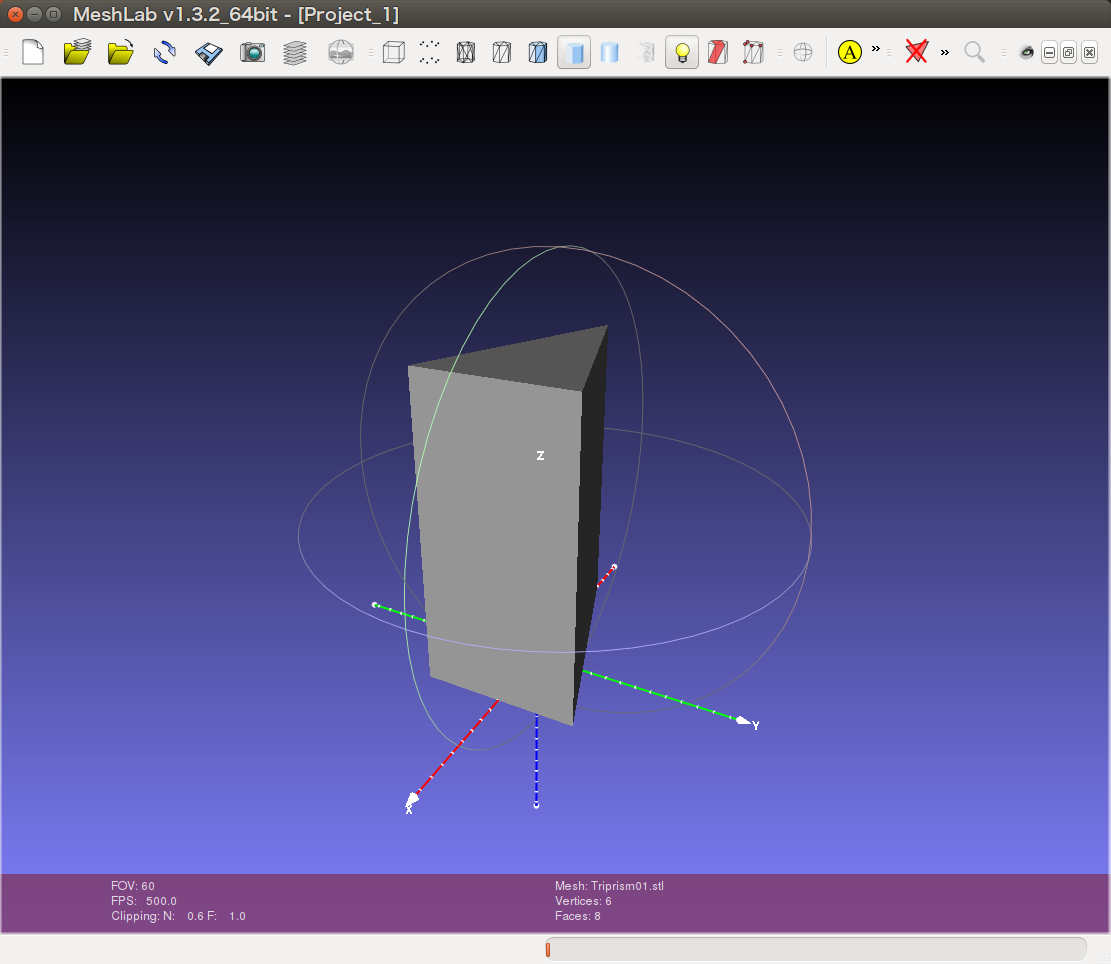
\includegraphics[width=100mm, bb = 0 0 1111 964]{fig/png/Triprism01.png}
  \caption{三角柱を作成した結果}
  \label{fig:三角柱を作成した結果}
\end{figure}

\subsection{課題2}
$O_1X_1Y_1Z_1$に四面体,$O_2X_2Y_2Z_2$に三角柱を,各任意座標系における初期位置に配置した結果をFig.~\ref{fig:四面体と三角柱を任意の座標系の初期位置に配置した結果}に示す.

\begin{figure}[t]
  \centering
  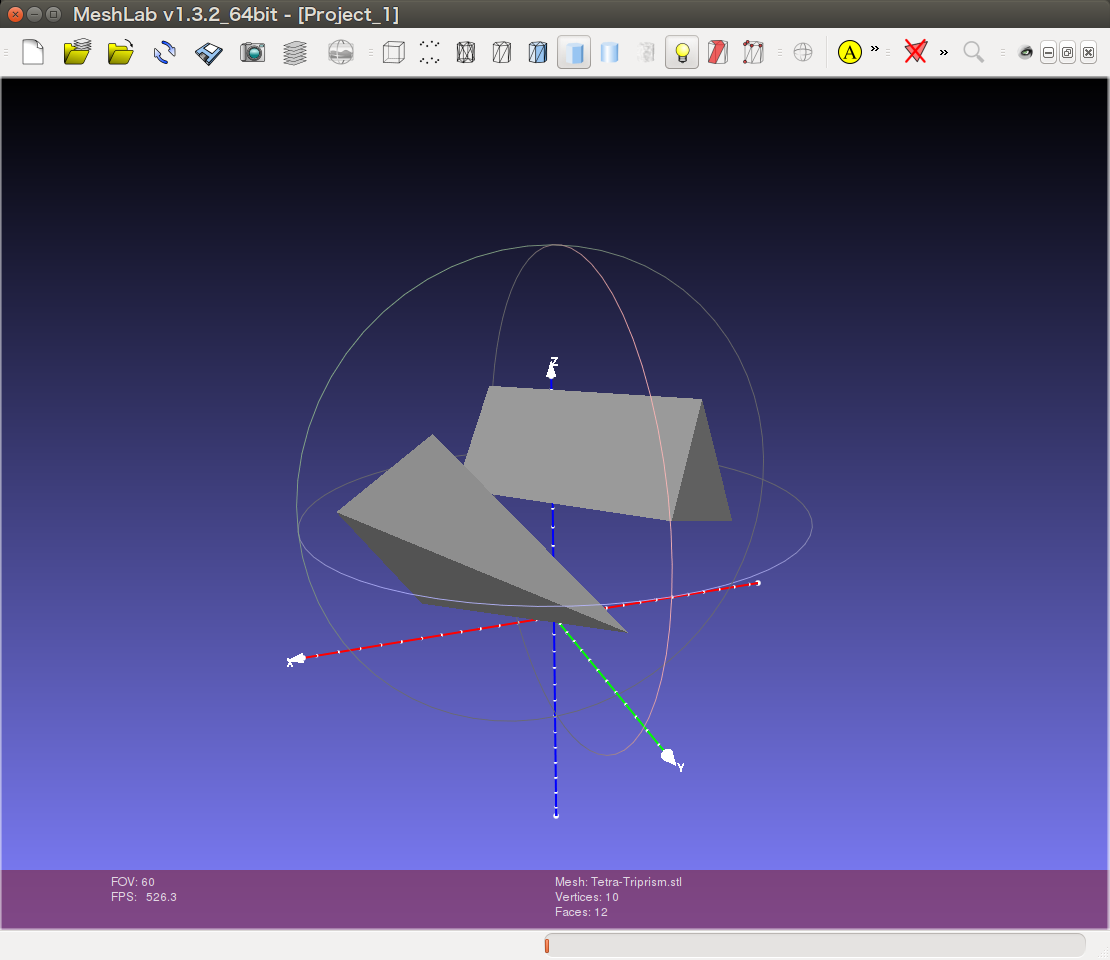
\includegraphics[width=100mm, bb = 0 0 1110 960]{fig/png/Tetra-Triprism.png}
  \caption{四面体と三角柱を任意の座標系の初期位置に配置した結果}
  \label{fig:四面体と三角柱を任意の座標系の初期位置に配置した結果}
\end{figure}
\end{document}